\documentclass[letterpaper, 11pt]{article}
\usepackage{import}
\import{../../../shared/config/}{packages}
\usepackage{graphicx}
\usepackage{float}
\usepackage[ruled, linesnumbered]{algorithm2e}

\import{../../../shared/config/}{styles}
\import{../../../shared/config/}{macros}

\title{Data Structures - Regular Grids}
\author{Zehua Chen}

\begin{document}
  \maketitle
  \tableofcontents

  \setmainstyles

  \section{Overview}

    A regular grid is an axis-alinged box, subdivided into smaller axis-aligned
    boxes called cells. Each cell have the same shape and size.

    \begin{itemize}
      \item Each cell contains a list of objects that
      \begin{enumerate}
        \item Are in the cell
        \item Are partially in the cell
        \item Maybe in the cell
      \end{enumerate}

      \item Grid will have $ O\left( \sqrt[3]{n} \right) $ in each axis
      \item In theory the ray will test on $ O\left( \sqrt[3]{n} \right) $
      objects, assuming one object per cell;
      \item In practice, $ O\left( \log n \right) $ tests per ray for a dense
      scene; rays typically stop early
    \end{itemize}

  \section{Construction}

    \begin{enumerate}
      \item Compute bounding boxes of all objects and construct a root
      bounding boxes that contain all of them
      \item Divide the root bounding boxes into cells
      \item Insert objects into the grid
    \end{enumerate}

    \paragraph{Implementation}

    \begin{itemize}
      \item Use a hash table
      \item Hash function (Morton Code) should map cells to an array index
      \item Only allocate space of a cell if it is occupied
    \end{itemize}

    \subsection{Morton Code}

      \begin{enumerate}
        \item Map point $ \left( x, y, z \right) $ into $ \left( i, j, k \right) $
        indices, i.e. grid cell address
        \item Convert $ \left( i, j, k \right) $ to binary
        \item Interleave the bits of the 3 binary numbers
      \end{enumerate}

    \subsection{How Many Cells}

      \begin{align}
        s &= \sqrt[3]{\frac{w_{x} w_{y} w_{z}}{n}} \\
        n_{x} &= \left\lfloor \frac{mw_{x}}{s} + 1 \right\rfloor \\
        n_{y} &= \left\lfloor \frac{mw_{y}}{s} + 1 \right\rfloor \\
        n_{z} &= \left\lfloor \frac{mw_{z}}{s} + 1 \right\rfloor
      \end{align}

      \begin{itemize}
        \item $ w_{x}, w_{y}, w_{z} $ are the lengths of the grid along each
        axis
        \item $ n_{x}, n_{y}, n_{z} $ are the number of cells along each axis
        \item $ n $ is the number of objects
        \item $ m $ allows us to pick how many cells per object
        \begin{itemize}
          \item $ m = 2 $ gives around 8 cells per object, good;
        \end{itemize}
      \end{itemize}

    \subsection{Put Objects into Cells}

      \begin{itemize}
        \item An AABB object has $ p_{o0}, p_{o1} $; root bounding box is
        defined by $ p_{g} $
        \begin{align}
          C\left( p_{o0} \right) &= \left( i_{0}, j_{0} \right) \\
          C\left( p_{o1} \right) &= \left( i_{1}, j_{1} \right) \\
          C\left( p_{o} \right) &= \frac{p_{o} - p_{g0}}{p_{g1} - p_{g0}} \\
          i &= \left\lfloor n C\left( p_{o} \right) \right\rfloor
        \end{align}

        Note that indices must be clamped in $ \left[ 0, n_{x} - 1 \right] $

        \item $ i, j $ are coordinates of cells
        \item Loop through all cells covered by $ C\left( p_{0} \right) $
        and $ C\left( p_{1} \right) $ and insert the object into each cell
      \end{itemize}

  \section{Traversing}

    \begin{algorithm}
      \caption{Traversing}
      \If{the ray misses the grid's bounding box} {
        \Return{false}\;
      }
      \If{the ray starts inside the grid's bounding box} {
        Find cell that contains the ray origin\;
      }
      \Else {
        Find the cell where the ray hits the grid from the outside\;
      }

      Traverse the grid\;
    \end{algorithm}

    \begin{itemize}
      \item Only test objects associated with cells traversed; all objects in
      cells must be tested
      \item Stops on the closest hit
      \item The ray's x, y, z increments will be uniform; we find the smallest
      $ t $ that will bring us into the next cell
    \end{itemize}

  \section{Mailboxing}

    \begin{figure}[H]
      \centering
      \caption{Mailboxing}
      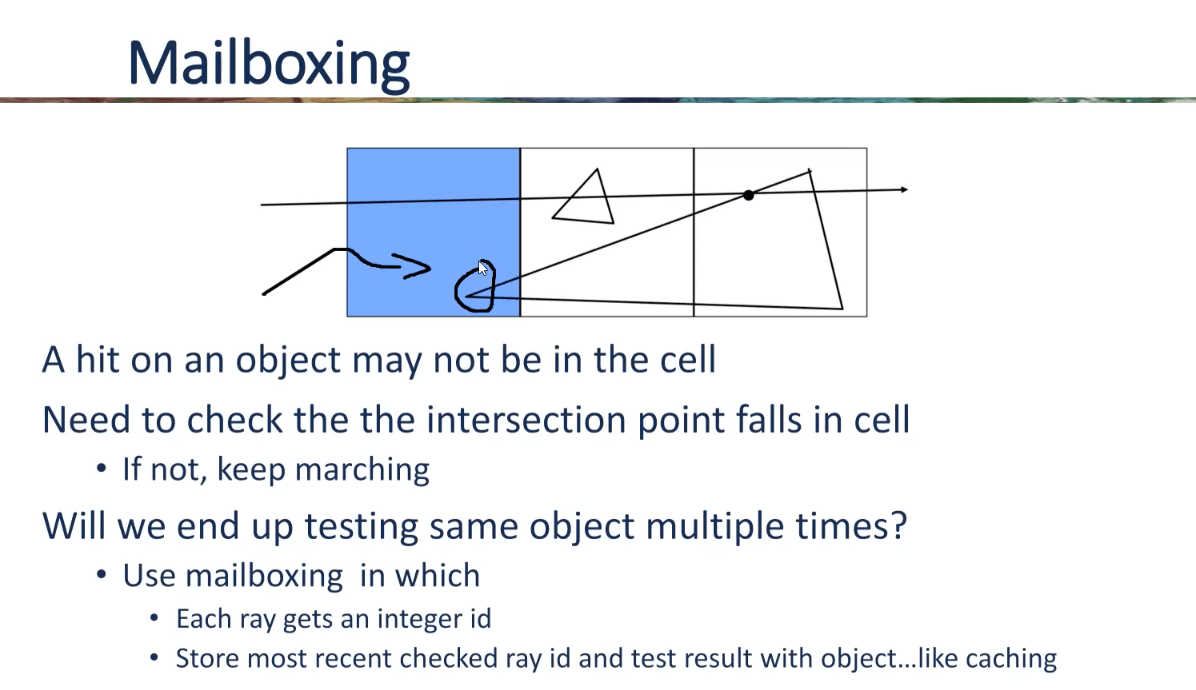
\includegraphics[width=0.7\columnwidth]{images/mailboxing.png}
    \end{figure}
\end{document}
